% Mirror: https://github.com/SIGma-UIUC/presentation-format
% --------------------------------------------------------------------
% This is a simple Beamer document that uses beamerthemesigma.sty
% Reading the comments should help you create a presentation even if
% you've never used Beamer before.
% --------------------------------------------------------------------

% Set our document class to Beamer
\documentclass[aspectratio=169, handout]{beamer}
% \documentclass[aspectratio=169, handout]{beamer}
% Add handout option to ignore pauses

% From Jeff E
\usepackage{algo}
% Some more macros
\usepackage{sigmastyle}
\usepackage{animate}


% Set a title
\title{Random Walks and Markov Chains}

% Set a subtitle if you desire
\subtitle{}

% Whoever worked on the presentation:
\author{Alex Jin}

% Date looks ugly, so leave blank
\date{}

% An institute name, if you're so inclined
% \institute{University of Illinois Urbana-Champaign}

% Use the SIGma theme for this Beamer presentation
\usetheme{sigma}
% --------------------------------------------------------------------

\newcommand{\pp}[0]{\mathbb{P}}
\newcommand{\ee}[0]{\mathbb{E}}

% Begin document
\begin{document}

% Beamer calls each slide a "frame", defined within the environment:
% \begin{frame}
%   <frame content here>
% \end{frame}

% This frame is just the title.
\begin{frame}
\titlepage
\end{frame}

\begin{frame}{Random Walks}
    \begin{center}
        \animategraphics[loop,controls,autoplay,width=150pt]{10}{rwanimate/rwanimate-}{1}{35}
        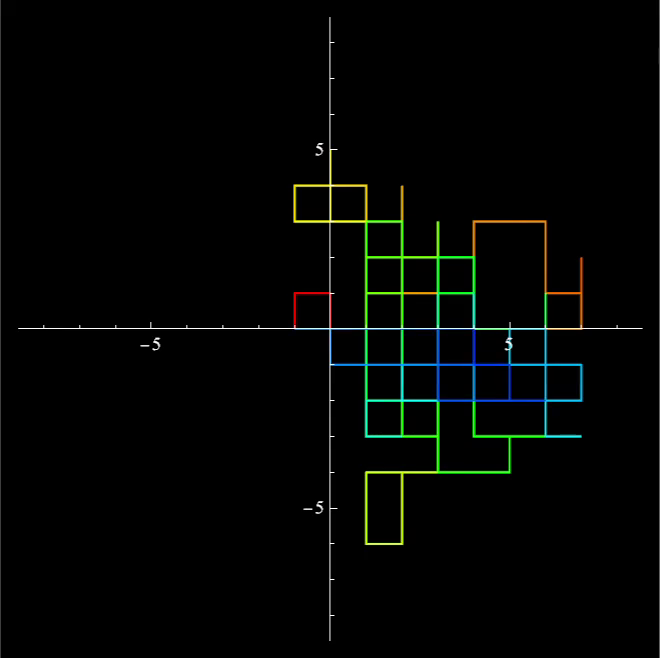
\includegraphics[width=150pt]{rwanimate/rwanimate-35.png}
    \end{center}
\end{frame}

\begin{frame}{More Random Walks}
    \begin{center}
        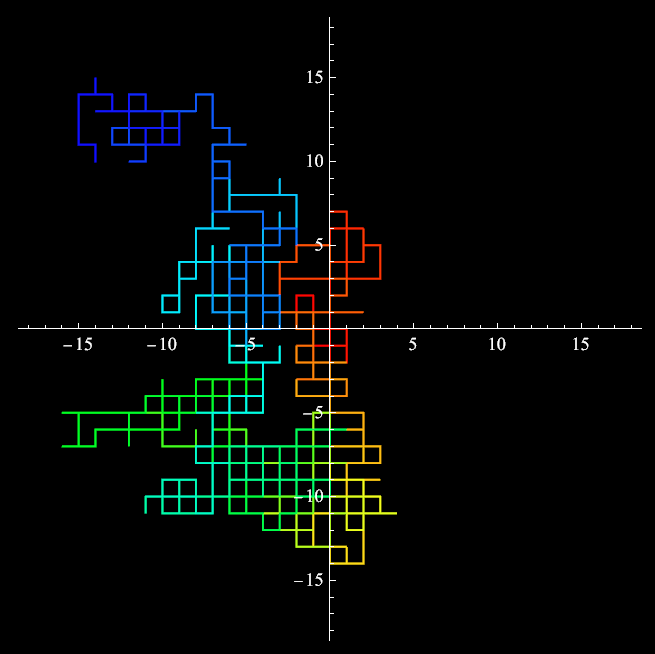
\includegraphics[width=150pt]{rws/rw0.png}
        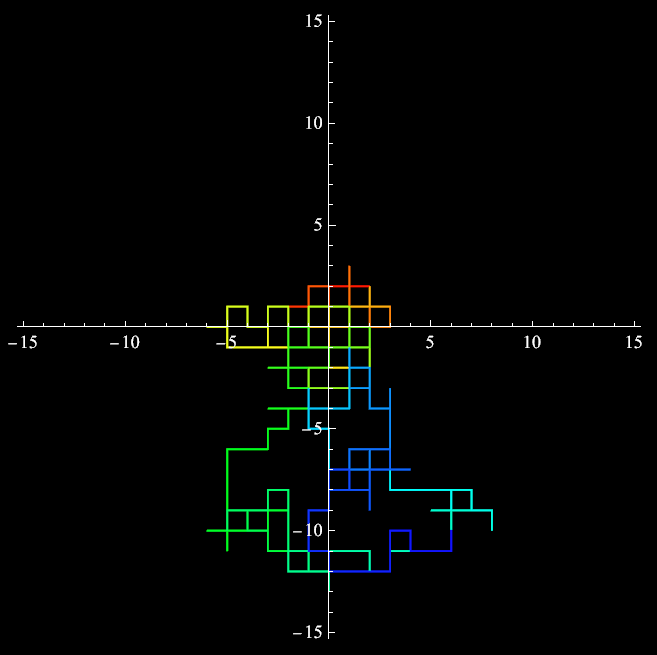
\includegraphics[width=150pt]{rws/rw00.png}
    \end{center}
\end{frame}

\begin{frame}{More Random Walks}
    \begin{center}
        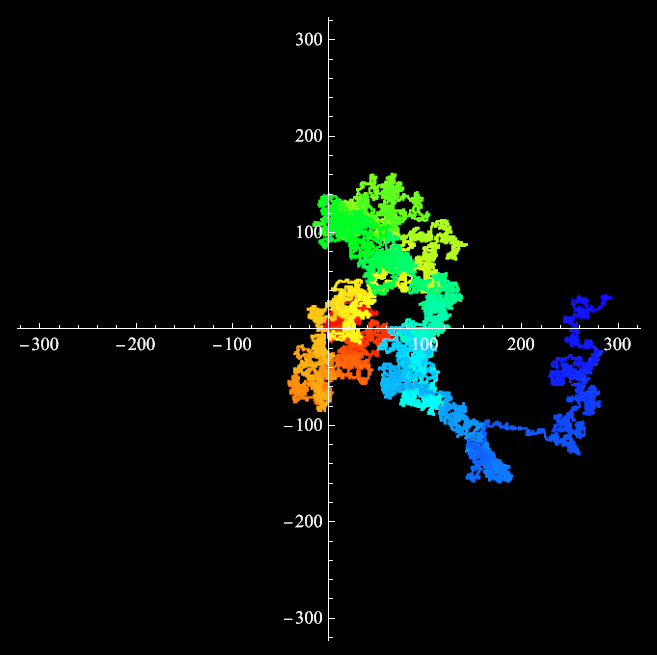
\includegraphics[width=110pt]{rws/rw1.png}
        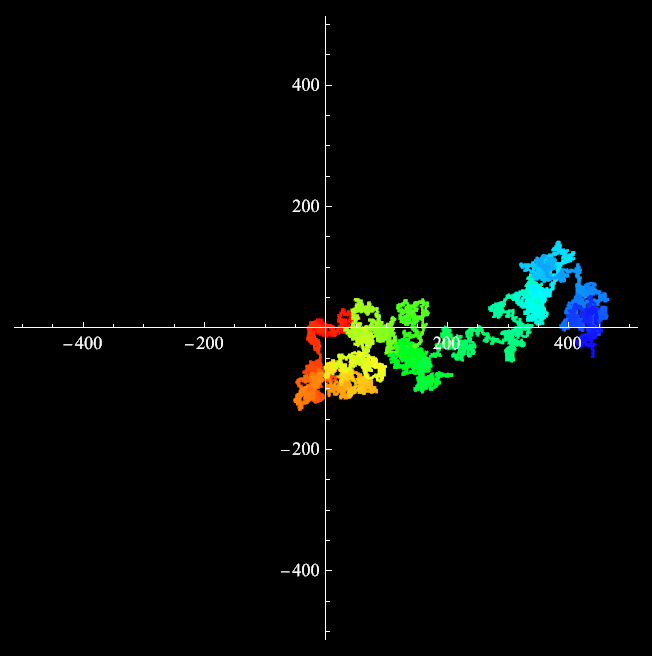
\includegraphics[width=110pt]{rws/rw2.png}
        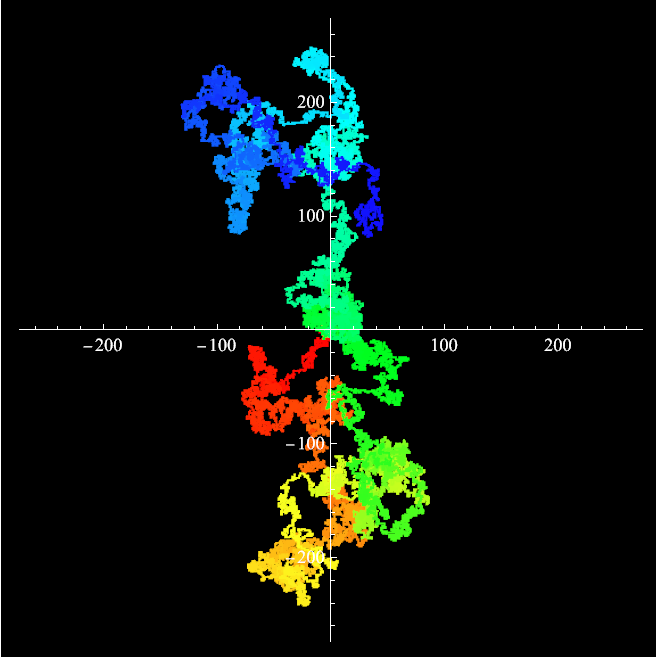
\includegraphics[width=110pt]{rws/rw3.png}
    \end{center}
\end{frame}
% Start a section: *sections* (subsections, etc.) are what show up in the TOC.
\section{Markov Chains}
% Section pages can be printed thus:
\frame{\sectionpage}
% There's a way to automate this, see:
% https://tex.stackexchange.com/questions/178800/creating-sections-each-with-title-pages-in-beamers-slides/178803

\begin{frame}{Definitions}
    \begin{itemize}
        \item A \textit{stochastic process} is a sequence of random variables 
        $[X_0,X_1,X_2,X_3,\dots]$ where $X_i \in \mathbb{Z}$.\pause
        \item If $X_t = i$, we say the process has value $i$ at time $t$. \pause
        \item A \textit{Markov Chain} is a random process with the Markov property:
    \end{itemize}
    \[ \pp(X_{t+1} = i_{t+1}~|~X_{t} = i_t,X_{t-1} = i_{t-1},\dots,X_0 = i_0)\]
    \[=\pp(X_{t+1} = i_{t+1}~|~X_{t} = i_t)\]
\end{frame}

\begin{frame}{Transition Probabilities}
  \begin{itemize}
      \item By the Markov property, the transition probabilities between any two states can be expressed as a single value:
      \[p_{ij} = \pp(X_{t+1} = j ~ | ~ X_t = i) \]
  \end{itemize}\pause
  \begin{thrm}
      A random process $(X_t)_{t\geq0}$ is Markov if and only if $\forall i_0,\dots,i_n$:
      \[\pp(X_1 = i_1,\dots,X_n = i_n ~|~X_0 = i_0) = p_{i_0i_1}p_{i_1i_2}\dots p_{i_{n-1}i_n} \]
  \end{thrm}
\end{frame}

\begin{frame}{Transition Matrix}
    The \textit{transition matrix} of a Markov Chain contains all transition probabilities:

    \[\begin{pmatrix}
        p_{00} & p_{01} & p_{02} & \dots\\
        p_{10} & p_{11} & p_{12} & \dots\\
        p_{20} & p_{21} & p_{22} & \dots\\
        \vdots & \vdots & \vdots & \ddots\\
    \end{pmatrix}\]
\end{frame}

\begin{frame}{Example: Random Walk on Number Line}
    Consider a symmetric random walk on the number line:
    \begin{center}
        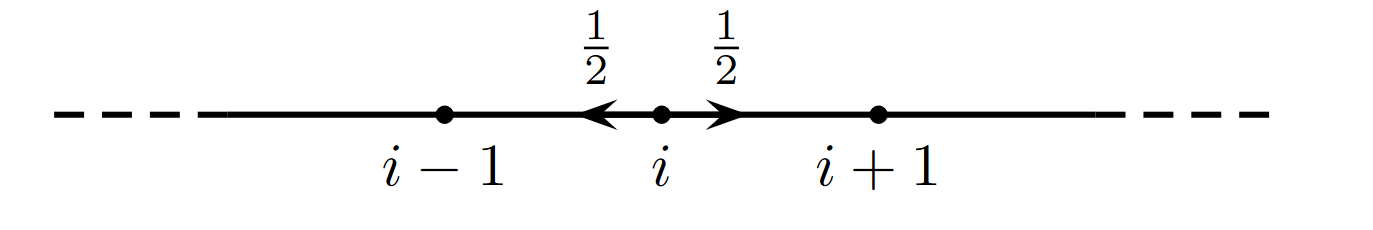
\includegraphics[width=300pt]{ssrw1d.png}
    \end{center}
    \pause
    \[\begin{pmatrix}
            & & \dots & \dots & \\
          & 0 & 1/2 & 0 & 0 & \\
        \dots & 1/2 & 0 & 1/2 & 0 & \dots\\
         \dots & 0 & 1/2 & 0 & 1/2 & \dots\\
         & 0 & 0 & 1/2 & 0 & \\
         & & \dots & \dots  &\\
    \end{pmatrix}\]
\end{frame}

\begin{frame}{Recurrence and Transience}
    \begin{itemize}
        \item We say state $i$ is \textit{recurrent} if, starting at $i$,
        \[\pp(\text{chain visits $i$ infinitely many times)} = 1\]
        \item We say state $i$ is \textit{transient} if, starting at $i$, 
        \[\pp(\text{chain visits $i$ infinitely many times)} = 0\]
    \end{itemize} \pause
    
https://illinois.zoom.us/j/84778016612?pwd=b0FDVWwxdDlMMjR4TzNqamo0ZGZKQT09    Ex. In the chain $\begin{pmatrix}
        0 & 1 \\
        0 & 1 
    \end{pmatrix}$, state 0 is transient, state 1 is recurrent.
\end{frame}

\begin{frame}{Recurrence and Transience}
    \begin{thrm}
        For a Markov Chain starting at $i$,\\
        \begin{enumerate}
            \item $\pp($chain eventually returns to $i) = 1 \Leftrightarrow$
        \[i \text{ is recurrent \& } \ee[ \text{number of visits to } i] = \infty,\]\pause
            \item $\pp($chain eventually returns to $i) < 1 \Leftrightarrow$
        \[i \text{ is transient \& } \ee[ \text{number of visits to } i] < \infty.\]
        
        \end{enumerate}\pause
    Goal: prove $(0,0)$ is a recurrent state in a random walk on $\mathbb{Z}^2$, and $(0,0,0)$ is a transient state in a random walk on $\mathbb{Z}^3$.
        
    \end{thrm}
\end{frame}

\section{A Proof}
\frame{\sectionpage}

\begin{frame}{Recurrence of 2-D Walk}
    Want to show: $\ee[$number of visits to (0,0)] = $\infty$.\pause
    \begin{pf}
        \begin{enumerate}
            \item Note that $\ee[$number of visits to (0,0)] = $\sum_{t=0}^\infty p_{00}^{(t)}$;\pause
            \item Since returning to the origin can only be accomplished with an even number of steps, we will only consider the even terms.\pause
            \item Then, 
            $
                p_{00}^{2t} = \frac{1}{4^t}\sum_{i=0}^t\frac{(2t)!}{i!i!(t-i)!(t-i)!}
                = \frac{1}{4^{2t}}{2t \choose t}\sum_{i=0}^t\frac{n!n!}{i!i!(t-i)!(t-i)!}$$ \pause
                = \frac{1}{4^{2t}}{2t \choose t}\sum_{i=0}^t{t \choose i}^2
                = \frac{1}{4^{2t}}{2t \choose t}^2
                \sim \frac{1}{\pi t}
            $ by Stirling's approximation. \pause
            \item Since $\sum p_{00}^{(t)} \sim \sum \frac{1}{\pi t}$, we may conclude that \pause both series diverge, hence (0,0) is recurrent.
        \end{enumerate}
    \end{pf}
\end{frame}

\begin{frame}{Transience of 3-D Walk}
    Want to show: $\ee[$number of visits to (0,0,0)] < $\infty$.\pause
    \begin{pf}
        \begin{enumerate}
            \item Note that $\ee[$number of visits to (0,0,0)] = $\sum_{t=0}^\infty p_{00}^{(t)}$;\pause
            \item Since returning to the origin can only be accomplished with an even number of steps, we will only consider the even terms.\pause
            \item Then, 
            $
                p_{00}^{2t} = \frac{1}{6^{2t}}\sum_{i+j+k=t}\frac{(2t)!}{(i!j!k!)^2}
                = \frac{1}{6^{2t}}{2t \choose t}\sum_{i=0}^t {t \choose i,j,k}^2
                $$ \pause
                \leq \frac{1}{6^{2t}}{2n \choose n}\sum_{i=0}^t{n \choose n/3,n/3,n/3}^2
                = \frac{1}{2^{2t}}{2n \choose n}{n \choose n/3,n/3,n/3}\frac{1}{3^t}
                \sim \frac{1}{2}\left(\frac{3}{\pi t}\right)^{3/2}
            $\pause
            \item Since $\sum p_{00}^{(t)} \leq \sum \frac{1}{2}\left(\frac{3}{\pi t}\right)^{3/2}$, we may conclude that \pause both series converge, hence (0,0,0) is recurrent.
        \end{enumerate}
    \end{pf}
\end{frame}

% Asking questions is fun but we should answer some first
\begin{frame}{}
      \begin{center}
    {\color{sigma@mainblue} \LARGE Questions?}
  \end{center}
\end{frame}

% Quotes are fun, find some to use!
\font\eightss=cmssq8
\font\eightssi=cmssqi8
\newcommand\quoteAuthorDate[2]{\begingroup
  \baselineskip 10pt
  \parfillskip 0pt
  \interlinepenalty 10000 % not needed in example
  \leftskip 0pt plus 40pc minus \parindent
  \let\rm=\eightss
  \let\sl=\eightssi
  \everypar{\sl}#1\par
  \nobreak\smallskip
  \noindent\rm--- #2\par
  \endgroup}
% If someone can figure out how to horizontally center this and make the text bigger that'd be cool
\begin{frame}{Acknowledgement}
    The material of this talk was adapted from MATH466 taught by Prof. Renming Song, with the proof taken from \cite{Norris_1997}.
\end{frame}

\begin{frame}
    \begin{center}
        \item \quoteAuthorDate{A drunk man will find his way home, but a drunk bird may get lost forever.}{Shizuo Kakutani}
    \end{center}
\end{frame}

% Remove this slide if you came up with all the material yourself
\begin{frame}[allowframebreaks]{Bibliography}
    \tiny
    \bibliography{refs}
    \bibliographystyle{alpha}
\end{frame}

\end{document}